\section{準備}
\label{section: preliminaries}

\subsection{表記}
(二進)自然数の集合を $\N$, 整数の集合を $\Z$, 実数の集合を $\R$, 
有理数の集合を $\Q$, $\T = \{0^n \mid n \in \N\}$ と表記する. 

$A \subset \R$ とする. 一変数関数 $f\colon A \to \R$ が $i$ 回微分可能であるとき,
その $i$ 階導関数を $\D{i}f$ と表記する.

二変数関数 $g \colon A \times B \to \R$ が
 $(i, j)$ 階連続的微分可能であるとき,
第一変数にたいして $i$ 階, 第二変数にたいして $j$ 階の導関数
はその微分の順序によらず等しい \cite{takagi1968analysis}.
よってその導関数を $\D{i,j}g$ と表記する.

実関数 $f \colon A \to \R$ にたいして $|f| = \max_{x \in A} f(x)$ と表記する.

\subsection{実数の名}
 実数は無限の長さを持つため, 有限な文字列に符号化することが不可能である.
 そこで文字列から文字列への関数に符号化する.
 \begin{definition}[実数の名]
  関数 $\phi \colon \T \to \Z $ が実数 $x \in [0,1]$ の名であるとは,
  $\phi(0^n) = \lfloor x \cdot 2^n \rfloor$ または
  $\phi(0^n) = \lceil x \cdot 2^n \rceil$ を満たすこと.
 \end{definition}
  ここで $\lfloor \cdot \rfloor, \lceil \cdot \rceil$ とはそれぞれ切り捨て関数と
 切り上げ関数である.
 つまり実数 $x$ の名とはサイズ $n$ の入力を受け取ると, $x$ の $n$ 桁精度を持つ
 近似値を返すような関数である.
 

\subsection{計算可能実関数, 多項式時間実関数}

 実関数は実数を受け取り, 実数を返す関数であるが,
 実数自体が関数として符号化されているため,
 実関数の計算する機械を神託機械として定義する.
 つまり関数の入力である実数の名を神託として与えられ,
 求める精度を入力として受け取ったとき,
 神託の表現する実数での関数の値の近似値を返すような神託機械を
 実関数を計算する機械と定義する[図 \ref{fig:model-of-function}].
 より厳密には以下のように定義する.

 \begin{figure}
  \label{fig:model-of-function}
  \begin{center}
   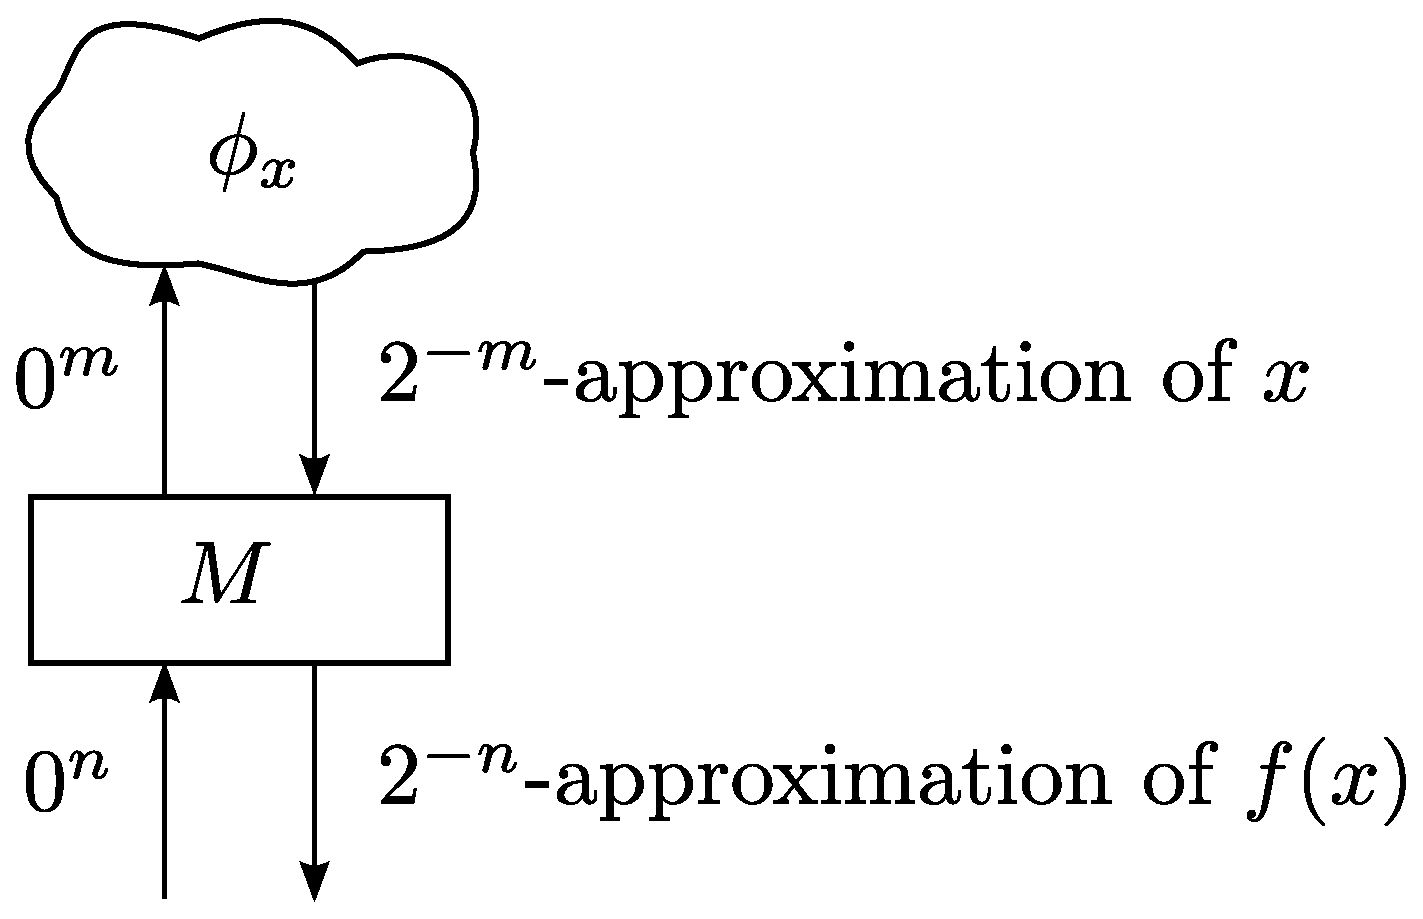
\includegraphics[height=0.15\textheight]{image/model-of-function.eps}
  \end{center}
  \caption{実関数のモデル化}
 \end{figure}

 \begin{definition}
  神託機械 $M$ が実関数 $f\colon A \to \R$ を計算するとは,
  任意の実数 $x \in A$, 任意の $x$ の名 $\phi_x$ にたいして,
  $M^{\phi_x}$ が $f(x)$ の名であること.
 \end{definition}
 計算可能な実関数は Grzegorczyk によって初めて形式的に定義され,
 \cite{grzegorczyk1955computable}.
 多変数関数のモデルも, 変数と同じ数だけ神託を持つ神託機械によって同様に定義される.

 ある実関数が計算可能であるとは, その関数を計算する神託機械が存在することである.
 同様に, ある実関数が多項式時間計算可能であるとは, その関数を計算する多項式時間神託機械が存在することである.

 神託機械 $M$ がある実関数族 $(f_u)_u$ を計算するとは,
 入力 $u$ を受けったとき, $M_u$ が $f_u$ を計算することである.
 実関数族が多項式時間計算可能であるとは, その実関数族を計算する
 多項式時間神託機械が存在することである.
 

 神託機械 $M$ で $f$ を計算するとき, 求める精度 $n$ にたいして,
 $x$ の近似値に必要な精度 $m$ が定まるため,
 計算可能な関数は連続である.
 また $n$ と $m$ の対応関係と有理数における近似値を与えることで,
 計算可能実関数や多項式時間計算可能実関数にたいして,
 神託機械を用いない同値な特徴付けが可能である.

 \begin{lemma}
  \label{lem:type1representation}
  実関数 $f\colon [0,1] \to \R$ にたいして,
  $\phi_f\colon (\Q \cap [0, 1]) \times \T \to \Q$, $m_f\colon \N \to \N$は
  \begin{align}
   |\phi_f(d, 0^n) - f(d)| \le 2^{-n} 
   &\qquad (d \in (\Q \cap [0,1]), \quad n \in \N)\\
   |x-y| \le 2^{-p_f(m)} \Rightarrow |f(x) - f(y)| \le 2^{-m}
   &\qquad (x, y \in [0, 1], \quad m \in \N)
  \end{align}
 をみたす関数とする.
  \begin{itemize}
   \item $f$ が計算可能であることは, 計算可能な $\phi_f, m_f$ が存在することと同値である. 
   \item $f$ が多項式時間計算可能であることは, 多項式時間計算可能な 
  $\phi_f$, 多項式 $m_f$ が存在することと同値である.
  \end{itemize} 
\end{lemma}

\subsection{完全性}

 関数の下限を示すために, 困難性及び完全性を定義する.
 言語 $L$ が実関数 $f\colon [0,1] \to \R$ に多項式時間還元可能であるとは,
 $f$ を計算する機械をブラックボックスとして, 入力 $u$ にたいして,
 精度を $f$ に与え, ある実数 $x_u$ の神託を模倣し, $f(x_u)$ の近似値から,
 $u$ が $L$ に含まれるか否かを多項式時間で計算可能であることである
 [図 \ref{fig:reduction}].
 厳密には以下のように定義する.

 \begin{definition}[多項式時間還元可能]
  言語 $L$ が実関数 $f\colon [0,1] \to \R$ に多項式時間還元可能であるとは, 
  任意の文字列 $u$ にたいして, 以下を満たす実数 $x_u \in [0,1]$
  多項式時間計算可能な関数 $R,S,T$ が存在すること.
  \begin{itemize}
   \item $R\colon N \times N \to \{0,1\}, \quad S\colon \N\times \T \to \N, \quad
  T\colon \N \to \T$;
   \item $S(u, \cdot)$ は実数 $x_u$ の名;
   \item 任意の $f(x_u)$ の名 $\phi$ にたいして
	 \[
	  L(u) = R(u, \phi(T(u))).
	 \]
  \end{itemize}
 \end{definition}

 \begin{figure}
  \begin{center}
  \label{fig:reduction}
  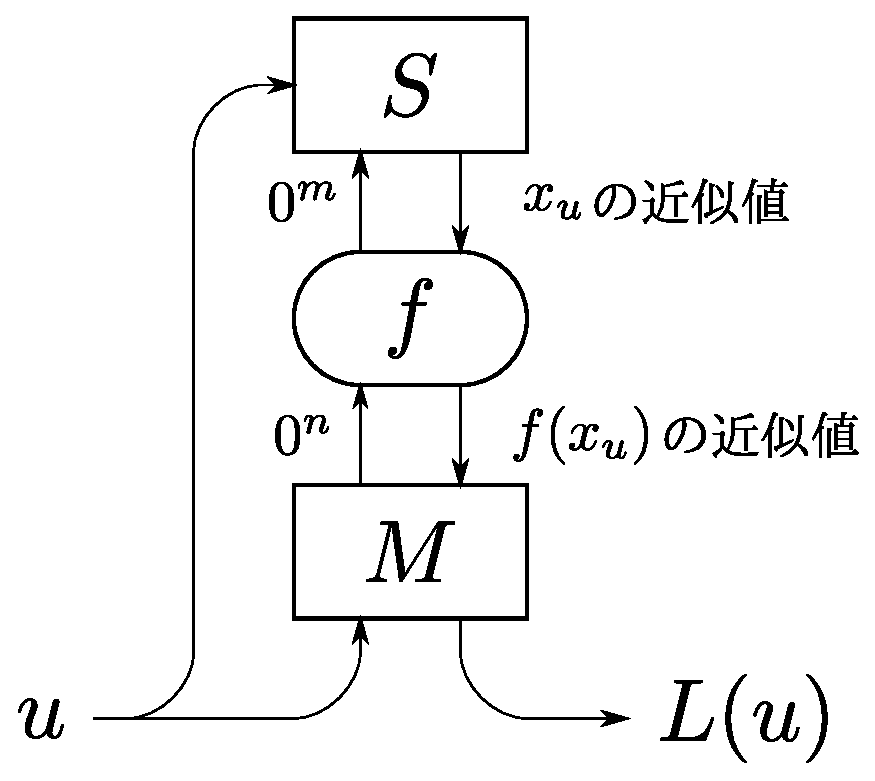
\includegraphics[height=0.2\textheight]{image/reduction.eps}
  \caption{言語 $L$ から関数 $f$ への還元}
  \end{center}
 \end{figure}

 計算量 $C$ にたいして, 関数 $f$ が $C$困難であるとは,
 任意の $C$ に含まれる言語が $f$ に多項式時間還元可能であることである.
 さらに $f$ が $C$ に含まれるとき, つまり $C$ に対応する神託機械で $f$ を計算するものが
 存在するとき, $f$ は $C$ 完全であると定義する.
 
